\documentclass[11pt,a4paper]{article}
\usepackage[utf8]{inputenc}
\usepackage[T1]{fontenc}
\usepackage{lmodern}
\usepackage{microtype}
\usepackage[a4paper,margin=1in]{geometry}
\usepackage{amsmath,amssymb}
\usepackage{booktabs,array,enumitem,tabularx}
\usepackage{graphicx}
\usepackage{pdfpages}
\usepackage{xcolor}
\definecolor{accent}{HTML}{1F3A5F}
\usepackage[colorlinks=true,linkcolor=accent,citecolor=accent,urlcolor=accent]{hyperref}
\usepackage{sectsty}
\usepackage{fancyhdr}
\usepackage{setspace}
\setstretch{1.15}
\sectionfont{\color{accent}\large}\subsectionfont{\color{accent}\normalsize}
\pagestyle{fancy}\fancyhf{}
\lhead{\small BS Project: Progress Report}\rhead{\small Prince Kumar (23B3032)}
\cfoot{\thepage}\renewcommand{\headrulewidth}{0.4pt}
\setlist{itemsep=1pt,topsep=3pt}

% numbers from the basis panel (filled from data/processed/basis_report.txt)
\newcommand{\basisN}{499{,}682}
\newcommand{\basisMedian}{1.2}
\newcommand{\basisPten}{$-33.0$}
\newcommand{\basisPninety}{26.1}
\newcommand{\vwapInRange}{99.8\%}

\begin{document}

\begin{center}
{\Large\bfseries\color{accent} Limits to Arbitrage in the Indian Equity Market}\\[4pt]
{\large Progress Report}\\[8pt]
Prince Kumar (23B3032), BS Economics, IIT Bombay\\
Guide: Prof.\ Aditi Chaubal \quad\textbar\quad EC 495 / EC 497\\
October 2026
\end{center}
\vspace{4pt}

\section{Summary}
Since the project document of September 2026, I have done five things.

\begin{enumerate}
\item \textbf{Checked and refined the plan.} I re-read the primary sources (the SEBI and NSE circulars and the core papers) and
corrected several institutional details in the project document. I also widened the framing: the project studies the limits
to arbitrage in Indian equities as a whole, and the F\&O ban is one of several sources of variation, not the only one.
\item \textbf{Built the theoretical framework you suggested.} One model covers all the limits the project studies (costs,
short-sale constraints, arbitrage capital, risk and position limits). The F\&O ban is modelled as the rule actually works.
The model changed parts of the empirical design. Section~\ref{sec:theory} gives a three-page summary and
Appendix~\ref{app:model} gives the full version.
\item \textbf{Built the ban and position-limit dataset} for every F\&O stock from February 2010 to October 2026, directly
from NSE archive files, and checked it against the exchange's rules.
\item \textbf{Built the price data and the main mispricing measure} (the futures-cash basis) for 2015 to 2026.
\item \textbf{Wrote down the tests before running them.} No mispricing measure has yet been compared with ban status, the
reforms or any other treatment. The hypotheses, designs and the results that would contradict them are fixed first
(Section~\ref{sec:tests}), so that the theory and the data cannot be adjusted to each other after the fact.
\end{enumerate}
Section~\ref{sec:plan} sets out the plan from here and Section~\ref{sec:questions} lists the points on which I would value
your guidance.

\section{Refinements to the project document}\label{sec:refine}
\subsection{Scope}
The research question is unchanged: how strongly do limits to arbitrage bind in Indian equities, and how much mispricing do
they explain? India offers a dated, observable shock to almost every kind of limit, which lets the project study them side by
side.

\begin{center}\small
\begin{tabularx}{\textwidth}{>{\raggedright\arraybackslash}p{3.3cm}>{\raggedright\arraybackslash}X}
\toprule
Kind of limit & Indian source of variation \\
\midrule
Short-sale constraints & Only F\&O-segment stocks are eligible for short selling and securities lending, and the practical
overnight short is the single-stock future. Entry into and exit from the F\&O segment changes this permanently; the F\&O ban
removes it temporarily. \\
Trading costs & Securities transaction tax (STT) on futures: 0.01\% from June 2013, 0.0125\% from April 2023, 0.02\% from
October 2024 and 0.05\% from April 2026. \\
Arbitrage capital and funding & Arbitrage mutual fund assets (large inflows after the April 2023 change in debt fund
taxation), money market rates, and the peak margin rules phased in from December 2020 to September 2021. \\
Arbitrage risk & Basis volatility and idiosyncratic volatility. \\
Position limits & The market-wide position limit (MWPL), entity limits, the ban rule, the March 2020 halving of the MWPL for
volatile stocks and the October 2025 change in the MWPL formula. \\
\bottomrule
\end{tabularx}
\end{center}

\subsection{Corrections to institutional details}
\begin{itemize}
\item \emph{Short selling.} The project document said there is no genuine short selling in the cash market. More precisely,
naked short selling is prohibited, short selling must be covered by delivery, and under SEBI's framework only securities in
the F\&O segment are eligible for short selling and stock lending. Retail traders can short within the day; overnight short
positions require stock lending, which is thin.
\item \emph{MWPL before October 2025.} The document gave the MWPL as 20\% of free float ``or 30 times the prior month's
volume''. The volume leg comes from a 2004 SEBI circular and was replaced in 2006 (SEBI/DNPD/Cir-31/2006). Throughout our
sample the MWPL was 20\% of free float, apart from the 2020 halving.
\item \emph{The ban rule.} A stock enters the ban when market-wide open interest exceeds 95\% of the MWPL at the end of a day,
and leaves it when open interest falls to 80\%. During the ban every participant may only reduce positions, rollovers into the
next expiry are not allowed, and from October 2025 the test uses delta-adjusted (futures-equivalent) open interest
(NSE Clearing circular 119/2025). Increases are penalised at 1\% of the value of the increase, subject to a minimum of
Rs 5,000 and a maximum of Rs 1 lakh per entity per stock per day.
\item \emph{The 2025 changes.} The document described the October and December 2025 changes as relaxations. In fact the new
formula, the lower of 15\% of free float and 65 times average daily delivery (measured in shares), with a floor of 10\% of free
float, lowered the MWPL of every F\&O stock (Section~\ref{sec:data}). The intraday checks of the MWPL from November 2025 are a
tightening. The effect on how often bans occur depends on each stock, because open interest is now also measured in delta terms.
\item \emph{Other points.} NSE sets the daily settlement price of a future at a theoretical cost-of-carry value when the
contract does not trade in the last half hour, which matters for measuring the basis. From August 2026 the closing price of
F\&O stocks comes from a closing auction. I could not find a source for the statement that position limits have been studied
in Korea and Taiwan, so I have dropped it.
\end{itemize}

\subsection{Changes to the design}
\begin{itemize}
\item \emph{Identification of the ban effect.} The project document proposed to use changes in the MWPL as an instrument for
ban status. The model shows why this does not work as stated: a change in the MWPL moves the chance of a future ban, and
traders respond to that chance even when no ban occurs. MWPL changes therefore identify the effect of the whole position-limit
regime. The effect of the ban itself is studied with designs built around the ban rule (Section~\ref{sec:tests}).
\item \emph{Mispricing measure.} The basis is built from daily volume-weighted prices of the future and the stock, not from
settlement prices, because of the theoretical settlement rule above.
\item \emph{Constraint index.} The index keeps its role as a stand-alone measure, but it is built only from frictions (costs,
lending, risk, position headroom). The basis and the ban, which are the outcome and the treatment, are no longer inputs.
\item \emph{Cross-section.} Besides the cross-sectional test of return signals, the project uses entry into and exit from the
F\&O segment. These events change the short-sale constraint for about two thousand listed stocks, which gives far more power
than the 200 or so F\&O stocks alone.
\item \emph{Earnings drift.} The earnings surprise is measured from the announcement-day return, which needs only prices.
Earnings per share would be added if a source is available through the library.
\item \emph{Put-call parity} is kept as a robustness check rather than a main measure, because many stock options trade thinly.
\end{itemize}

\section{Theoretical framework: summary}\label{sec:theory}
\subsection{Set-up}
The \emph{basis} is the gap between the futures price and its cost-of-carry value, $m=\ln F-\ln F^*$, with
$F^*=(S-\mathrm{PV}(D))e^{r(T-t)}$. Outside traders trade the stock and the future. Their demands depend on prices and on a
demand shifter, so that without arbitrage the basis equals $u/\Phi$, where $u$ is the relative demand pressure toward futures
and $\Phi$ measures the depth of the two markets. An arbitrage sector holds $a$ units of the cash-and-carry trade (long stock,
short future). Market clearing gives
\[
m=\frac{u-a}{\Phi}.
\]
Arbitrageurs choose $a$ to maximise $am-\tfrac{\gamma}{2}a^2-c_+a^+-c_-a^-$. Here $\gamma=\alpha\sigma^2$ reflects risk
aversion per unit of capital and the risk of the basis before convergence, $c_+$ is the cost of a cash-and-carry position and
$c_-$ the cost of a reverse position, which needs stock lending. Each Indian limit enters as a parameter: costs (STT, fees,
funding) through $c_\pm$, short-sale constraints through $c_-$, capital and risk through $\gamma$, and position limits through
caps on $a$.

\subsection{The no-arbitrage band}
Arbitrage starts only when the basis leaves the band $[-c_-,\,c_+]$. Inside the band the basis moves one-for-one with demand;
outside it arbitrage absorbs part of every shock. This gives four implications.
\begin{itemize}
\item Costs set the edges of the band, so a change in STT should move the edges by about the change in cost.
\item Capital and risk set how far the basis travels beyond an edge.
\item The edges shrink as expiry approaches.
\item Because reverse arbitrage is expensive in India, the band sits below zero. Earlier Indian studies find exactly this.
\end{itemize}
When arbitrageurs already hold positions, the range in which they do not trade is
$[\gamma a_{t-1}-c_u,\ \gamma a_{t-1}+c_+]$, where $c_u$ is the cost of unwinding. The thresholds therefore move with the size
of existing arbitrage positions. This matters for the threshold models used in the estimation.

\subsection{The F\&O ban}
In a ban every participant, not only arbitrageurs, may only reduce positions. Two consequences follow.

\emph{First, arbitrage becomes one-sided.} Arbitrageurs cannot open new cash-and-carry positions, so a future that is too rich
is no longer corrected. They can still unwind existing positions (sell the stock, buy back the future), so a future that is
too cheap is still corrected, at a floor $\gamma a_t-c_u$ that rises with the remaining positions. The floor wears out as
positions are unwound, and an expiry inside the ban removes positions that cannot be rolled over.

\emph{Second, demand for new futures exposure is blocked.} Part of it moves to the cash market (for example, a trader who
cannot buy the future buys the stock on margin). This reverses the sign of the response of the basis: in normal times new long
demand raises the basis, in a ban it lowers it.

Together these imply that the effect of a ban on the \emph{level} of the basis has no fixed sign. It is positive when the
pressure comes from traders closing positions and negative when new speculative demand keeps arriving. The empirical test is
therefore whether the sign follows the composition of trading, not whether bans ``widen'' mispricing.

\subsection{Other implications}
\begin{itemize}
\item \emph{Trading in a ban.} Every trade closes a long and a short position, so the change in open interest should equal
minus the volume, and futures trading should thin out. On days without trades NSE's theoretical settlement price makes a
settlement-based basis zero by construction.
\item \emph{Anticipation.} If exit is costlier during a ban, arbitrageurs ask for a higher return before opening positions as
utilisation approaches 95\%. The band widens smoothly before a ban, so a regression discontinuity at 95\% captures only part of
the effect.
\item \emph{The MWPL as an instrument.} Because the MWPL affects the chance of a future ban, it affects the basis even on days
without a ban. It is not a valid excluded instrument for ban status.
\item \emph{Earnings news.} In a ban, informed traders cannot short through futures, so bad news is absorbed more slowly and
the drift after bad news should be larger. Good news can still be traded in the cash market.
\item \emph{F\&O entry.} Following Miller (1977), when investors disagree and cannot short, prices reflect the optimists. The
model gives the overpricing in closed form; it rises with disagreement and falls when shorting becomes possible. Entry into
the F\&O segment should therefore lower overpricing, more so for stocks with high disagreement.
\end{itemize}
All closed-form results were checked numerically, and a simulation of the dynamic version reproduces the one-sided correction
during bans.

\section{Data built so far}\label{sec:data}
\subsection{Sources}
All data come from free NSE archive files, downloaded and parsed with scripts so that every step can be repeated.
\begin{center}\small
\begin{tabularx}{\textwidth}{>{\raggedright\arraybackslash}p{4.2cm}>{\raggedright\arraybackslash}X>{\raggedright\arraybackslash}p{3.1cm}}
\toprule
File & Content & Coverage \\
\midrule
Combined open interest (daily) & MWPL, open interest, delta-adjusted open interest (from October 2025), status for the next day & Feb 2010 to Oct 2026 \\
Securities in ban (daily) & Official ban list & Feb 2010 to Oct 2026 \\
F\&O bhavcopy (daily) & Futures prices, traded value, contracts, open interest; options activity by stock & 2015 to 2026 \\
Cash bhavcopy and delivery file (daily) & Prices, traded value and quantity, delivery quantity & 2015 to 2026 \\
Corporate actions & Dividends, splits and bonus issues with ex-dates & 2014 to 2026 \\
Interest rates & Three-month interbank rate (monthly) & 2011 to 2026 \\
\bottomrule
\end{tabularx}
\end{center}

\subsection{Checks}
Before using the data I checked them against the exchange's own rules and against each other.
\begin{itemize}
\item The daily ``no fresh positions'' flags agree with the next day's official ban list in 99.85\% of cases. Each remaining
difference traces to a dated NSE file that carries another day's data, to a corrupt NSE file or to a special session.
\item The ban rule holds in the data: utilisation was above 95\% on the day before 99.2\% of ban spells began, and at or below
80\% on the last day of 99.5\% of spells.
\item The set of stocks in the open interest files matches the set of stock futures in the F\&O bhavcopy exactly.
\item Some NSE files needed care: about a hundred files write the year in two digits, a few carry another day's data under
their own date, and some zip files bundle several days. The parsing handles all of these, and every correction is logged.
\item Known gaps at the source: 13 corrupt open interest files in May and June 2012 (before the main sample) and the F\&O
bhavcopy of 30 March 2021.
\end{itemize}

\subsection{First facts on bans}
Table~\ref{tab:bans} summarises the bans from 2015. Over 2015 to 2026 there were 1,789 ban spells covering 9,414 stock-days
and 141 stocks. Bans were most frequent in 2017 and 2024. A typical spell lasted four trading days up to September 2025.
Under the new rules spells are fewer but longer: the 44 spells since October 2025 have a median length of nine days.

\begin{table}[h]
\centering\small
\caption{F\&O bans by year, 2015 to 2026}\label{tab:bans}
\begin{tabular}{lrrrrrr}
\toprule
Year & \shortstack[r]{F\&O stocks\\(avg per day)} & \shortstack[r]{Stocks\\banned} & \shortstack[r]{Ban\\spells} & \shortstack[r]{Ban\\stock-days} & \shortstack[r]{Median spell\\(days)} & \shortstack[r]{Longest spell\\(days)} \\
\midrule
2015 & 154 & 16 & 69 & 367 & 4 & 21 \\
2016 & 172 & 27 & 136 & 645 & 4 & 17 \\
2017 & 201 & 43 & 287 & 1586 & 5 & 24 \\
2018 & 206 & 38 & 162 & 810 & 4 & 31 \\
2019 & 176 & 23 & 86 & 508 & 4 & 17 \\
2020 & 140 & 40 & 178 & 756 & 3 & 13 \\
2021 & 163 & 26 & 162 & 789 & 4 & 16 \\
2022 & 196 & 23 & 100 & 457 & 4 & 13 \\
2023 & 187 & 41 & 193 & 942 & 4 & 17 \\
2024 & 185 & 49 & 289 & 1656 & 5 & 22 \\
2025 & 216 & 37 & 94 & 556 & 5 & 15 \\
2026$^{a}$ & 209 & 10 & 33 & 342 & 10 & 29 \\
\midrule
2015 to 2026 & 183 & 141 & 1789 & 9414 & 4 & 31 \\
\bottomrule
\end{tabular}


\vspace{3pt}{\footnotesize $^{a}$ January to 27 October 2026. Spells are counted in the year they start.}
\end{table}

\begin{figure}[h]
\centering
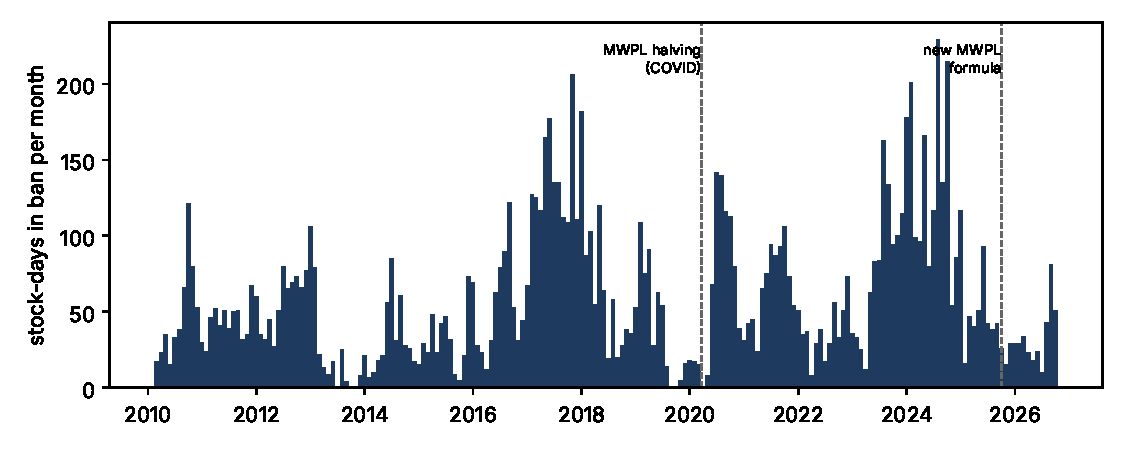
\includegraphics[width=0.9\textwidth]{../reports/figs/ban_days_per_month.pdf}
\caption{Stock-days in the F\&O ban per month, 2010 to 2026.}
\end{figure}

\subsection{Changes in the MWPL}
\begin{itemize}
\item \emph{March 2020.} The MWPL was halved for 61 stocks between 20 and 27 March 2020 and restored for 70 stocks on
26 November 2020. These dates match the regulatory record.
\item \emph{October 2025.} On 1 October 2025 the new formula lowered the MWPL of all 208 F\&O stocks (Figure~\ref{fig:mwpl}).
The median stock's limit fell to 73\% of its old value. 17\% of stocks are at the floor (half the old limit) and 48\% at 15\% of
free float (three quarters of the old limit). Because the size of the cut differs across stocks and was set by data from before
the reform, it can be used as a measure of treatment intensity.
\item \emph{Regular updates.} Outside these events the MWPL changes mainly in February, May, August and November, when free
float is updated from quarterly shareholding filings.
\end{itemize}

\begin{figure}[h]
\centering
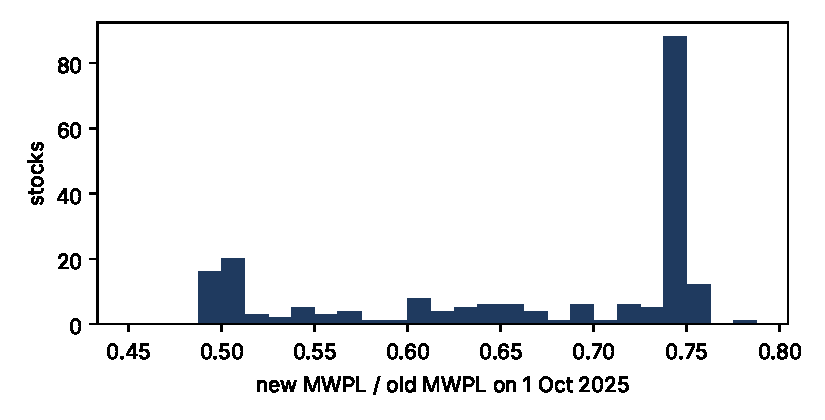
\includegraphics[width=0.62\textwidth]{../reports/figs/mwpl_ratio_oct2025.pdf}
\caption{Ratio of the new to the old MWPL on 1 October 2025, all F\&O stocks.}\label{fig:mwpl}
\end{figure}

\begin{figure}[h]
\centering
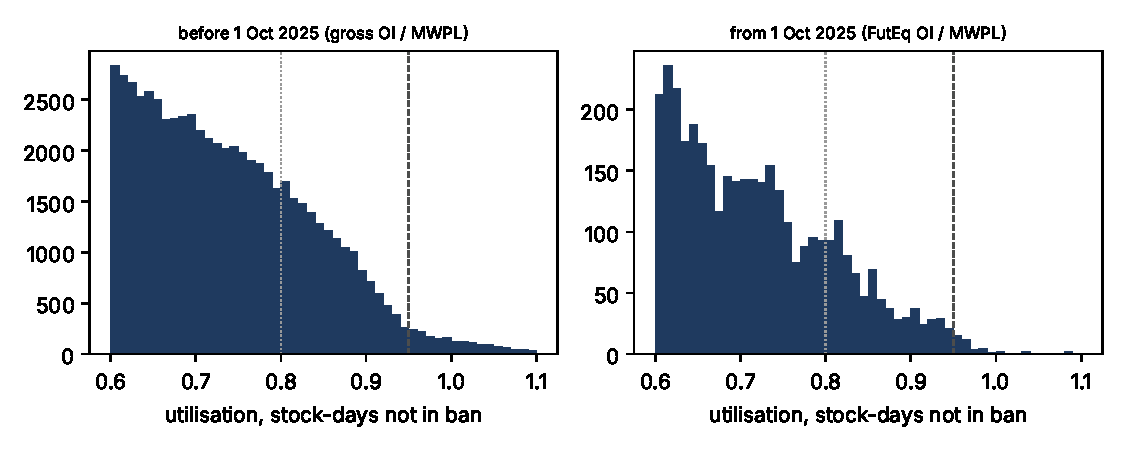
\includegraphics[width=0.9\textwidth]{../reports/figs/utilisation_near_threshold.pdf}
\caption{Utilisation of the MWPL on days a stock is not in a ban. Dashed line: 95\% entry threshold; dotted line: 80\% exit
level.}\label{fig:util}
\end{figure}

Figure~\ref{fig:util} shows how utilisation is distributed near the 95\% threshold. Before the reform the density thins out
smoothly through 95\%, with no visible pile-up just below it. A formal density test comes before any regression
discontinuity analysis.

\subsection{The mispricing measure}
For each stock and day the basis is computed from the volume-weighted average prices of the near-month future and of the
stock, net of dividends going ex before expiry and of the cost of carry at the three-month interbank rate. The older F\&O files
do not report lot sizes, so lot sizes are recovered from open interest and checked against the day's price range: the futures
average price lies within the day's high and low for \vwapInRange\ of traded contracts. Every futures observation has a
matching cash price, and the trading days in the price files match those in the open interest files exactly.

Two checks led to changes. First, some corporate events other than dividends (for example the bonus debentures issued by NTPC
in March 2015) move the futures price relative to the stock. Days on which such an event, or a dividend, goes ex before expiry
are flagged and kept out of the main sample. Second, adjusting for dividends with their actual ex-dates over-corrects a little,
probably because some dividends were not yet announced on the earlier days; these days are also flagged.

On the remaining \basisN\ stock-days with at least five contracts traded, the median basis is \basisMedian\ basis points, and
the 10th and 90th percentiles are \basisPten\ and \basisPninety\ basis points. The basis shrinks toward expiry, and its
distribution is stable across the change in NSE's file format in July 2024. About 0.7\% of stock-days lie more than 200 basis
points from zero. These come mainly from stocks under heavy selling pressure (for example during business or credit distress),
not from data errors, so they are kept and handled with the estimation methods. A comparison of the index futures basis with
money market rates is still to be done, because it needs index dividends: the implied rate on Nifty futures is lowest every
July to September, when most index dividends are paid. As noted above, no mispricing measure has yet been related to bans,
reforms or other treatments.

\section{Pre-specified tests}\label{sec:tests}
The main hypotheses, how each will be tested and what result would contradict it:
\begin{center}\small
\begin{tabularx}{\textwidth}{>{\raggedright\arraybackslash}p{3.3cm}>{\raggedright\arraybackslash}X>{\raggedright\arraybackslash}X}
\toprule
Hypothesis & Design & Contradicted if \\
\midrule
Bans make correction one-sided & Ban-entry event study against stocks that came close to 95\% but did not cross; threshold
models with ban-dependent adjustment & Positive and negative deviations change in the same way, or not at all \\
Bans move trading out of futures & Change in open interest against volume; futures and cash volume, delivery share & No change in futures activity \\
Costs set the band edges & Event windows around the STT changes of 2023, 2024 and 2026 & Edges unrelated to the size of the cost change \\
Short-sale access lowers overpricing & Staggered difference-in-differences around F\&O entry and exit, with matched controls & No change or the opposite sign \\
Position-limit regime & Continuous treatment intensity from the October 2025 formula; quarterly MWPL resets; behaviour as utilisation approaches 95\% & No gradient before 95\%, or no effect of the predicted change in utilisation \\
Level effect of bans & Ban-entry event study split by the composition of trading before the ban & Sign unrelated to the composition \\
\bottomrule
\end{tabularx}
\end{center}
Secondary hypotheses cover the constraint index, earnings drift in bans, arbitrage capital and return signals. Inference uses
standard errors clustered by stock and date, with a correction for testing several main hypotheses. Power is an issue for the
post-reform period, which has only 44 ban spells; results for that period will be reported with this caveat.

\section{Plan from here}\label{sec:plan}
The steps below are in order of dependence.
\begin{enumerate}
\item Finish the price data: add the list of F\&O entries and exits, the free-float history, the announcement dates for
results and the dividends of the Nifty index, and compare the index futures basis with money market rates.
\item Fix the test plan in writing, including sample filters, variable definitions and specifications, before any outcome is
related to a treatment.
\item Estimate the no-arbitrage band with three-regime threshold error-correction models and smooth-transition models, and
relate the band to the dated cost and capital changes.
\item Estimate the effects of the ban: event study, hysteresis comparison between 80\% and 95\% utilisation, regression
discontinuity at 95\% (as supporting evidence) and the October 2025 reform.
\item Estimate the effects of F\&O entry and exit, and the cross-sectional test of return signals.
\item Build and validate the constraint index.
\item Write the policy chapter and the thesis, and release the code and the derived measures so the work can be reproduced.
\end{enumerate}

\section{Points on which I would value your guidance}\label{sec:questions}
\begin{enumerate}
\item Is the wider framing (limits to arbitrage in general, with the ban as one source of variation) acceptable to you?
\item Is the theoretical framework at the right depth for the thesis, or should parts of it be simplified or extended?
\item For the band estimation, would you prefer the three-regime threshold models, the smooth-transition models, or both? I
would also welcome your advice on threshold models in which the thresholds depend on an observed state (existing arbitrage
positions, or whether a stock is in a ban).
\item Can the department or library give access to a database with earnings per share and shareholding history (for example,
CMIE Prowess)?
\item Would you like the test plan sent to you before I run the main estimates?
\end{enumerate}

\section*{References}
\small
\begin{description}[leftmargin=1.2em,itemsep=0pt,font=\normalfont]
\item Aggarwal, N. (2015). Limits to arbitrage: The case of single stock futures and spot prices. IGIDR Working Paper WP-2015-010.
\item Gromb, D. and D. Vayanos (2010). Limits of arbitrage. \emph{Annual Review of Financial Economics} 2, 251-275.
\item Miller, E. (1977). Risk, uncertainty, and divergence of opinion. \emph{Journal of Finance} 32(4), 1151-1168.
\item NSE Clearing (2025). Circular 119/2025 (8 September 2025) and FAQ on position limits and securities in the ban period (13 October 2025).
\item SEBI (2006). Circular SEBI/DNPD/Cir-31/2006 on the market-wide position limit.
\item SEBI (2025). Circular SEBI/HO/MRD/TPD-1/P/CIR/2025/79, 29 May 2025.
\item Shankar, R.L., G. Sankar and K. Kiran Kumar (2019). Mispricing in single stock futures: Empirical examination of Indian markets. \emph{Emerging Markets Finance and Trade} 55(7), 1619-1633.
\item Shleifer, A. and R. Vishny (1997). The limits of arbitrage. \emph{Journal of Finance} 52(1), 35-55.
\item Ters, K. and J. Urban (2020). Estimating unknown arbitrage costs: Evidence from a 3-regime threshold vector error correction model. \emph{Journal of Financial Markets} 47, 100503.
\item Tse, Y. (2001). Index arbitrage with heterogeneous investors: A smooth transition error-correction analysis. \emph{Journal of Banking and Finance} 25(10), 1829-1855.
\end{description}

\appendix
\clearpage
\section{Theoretical framework: full version}\label{app:model}
The following pages give the full model with proofs, the numerical checks and the mapping from results to hypotheses.
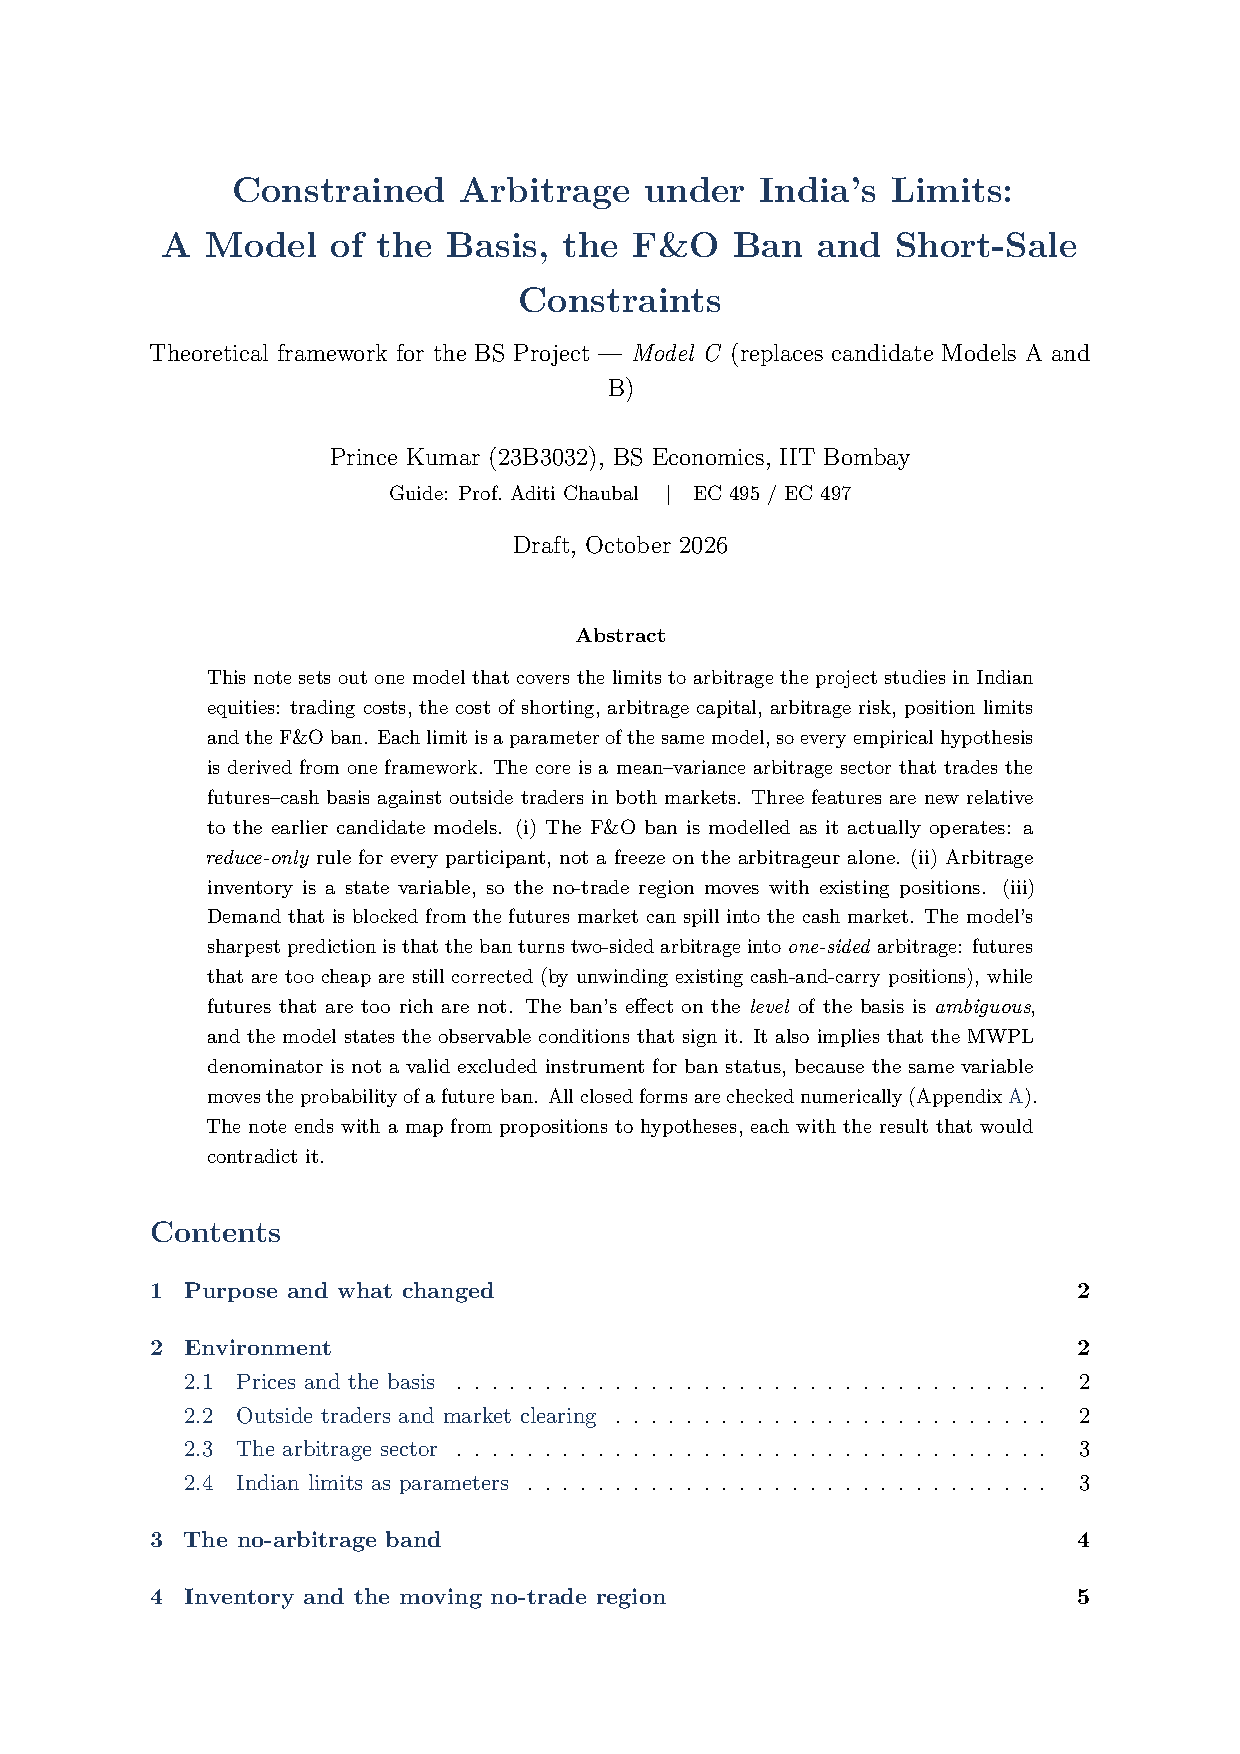
\includepdf[pages=-,pagecommand={\thispagestyle{empty}}]{../BSP_Model_C_Constrained_Arbitrage_India.pdf}

\end{document}
